% Vorlage verwenden. ACHTUNG der Pfad ist relativ und geht davon aus, 
% diese Datei zwei Ordnerebenen höher liegt als Vorlagen
\newcommand*{\VorlagenPfad}{../../Vorlagen}%
\documentclass{\VorlagenPfad/coderdojokatext}
\usepackage{graphicx}

% Titel als Kommando für den Header/Footer definieren
\newcommand{\Titel}{Rechtecke malen}

\begin{document}
	
	\begin{center}
		{\huge \Titel}
	\end{center}
	
	\section{Die Aufgabenstellung} Donald Duck hat ein neues Hobby entdeckt: das Malen! Da er aber etwas tollpatschig ist, malt er besonders gerne Bilder, die aus geometrischen Figuren, wie Rechtecken oder Kreisen bestehen.
	\\
	\begin{figure}[h]
	\caption{Eines von Donalds Bildern.}
	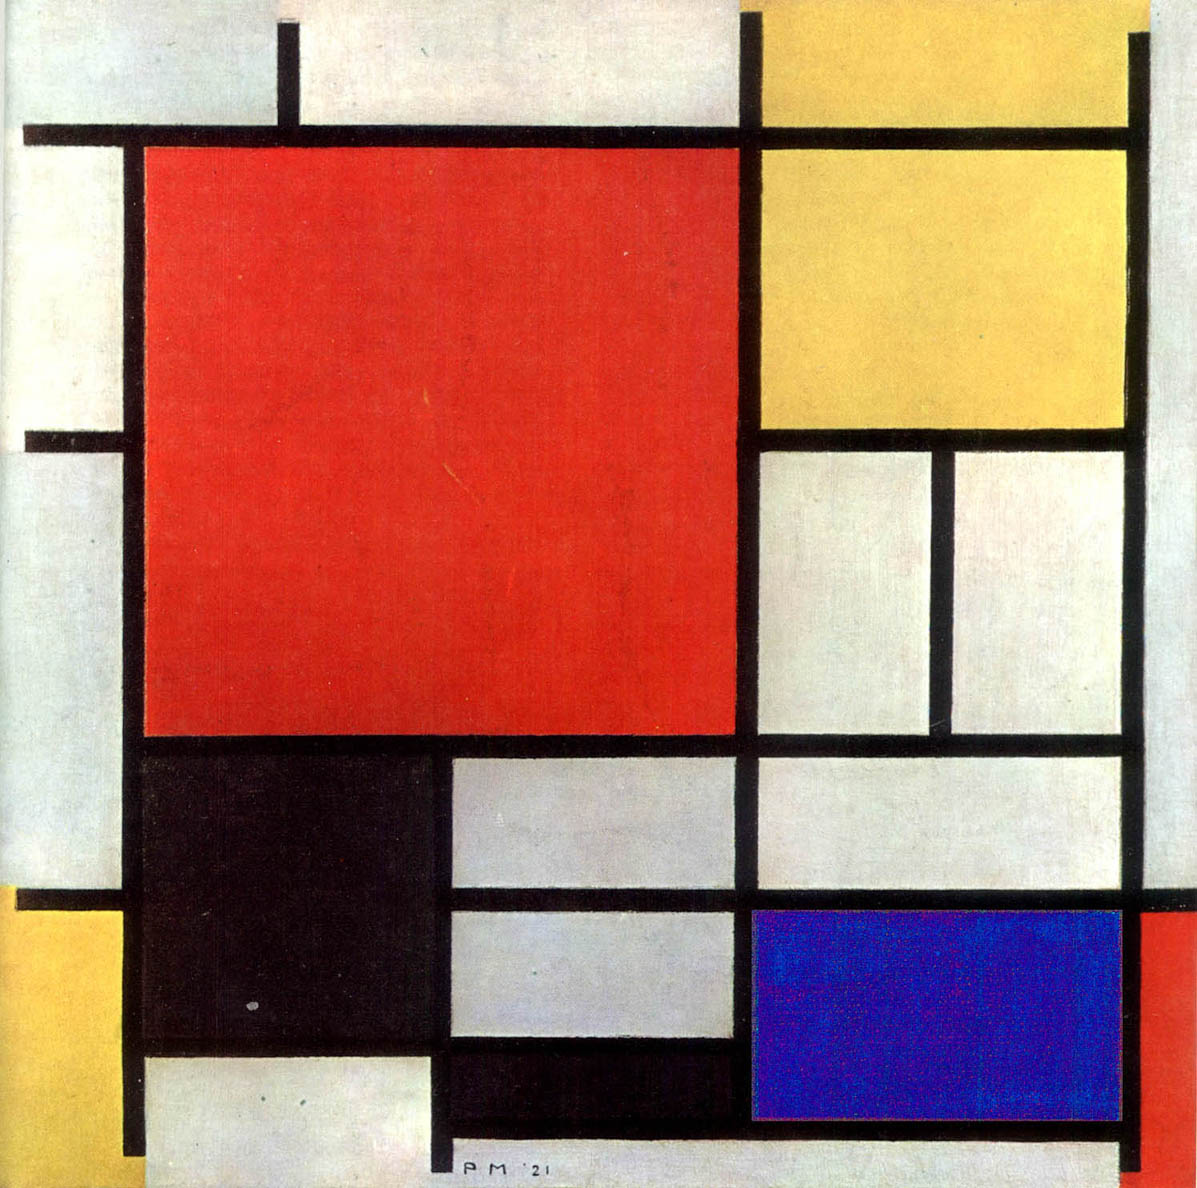
\includegraphics[scale=0.3]{Piet}
	\centering
	\end{figure}
	\\ \\
	Nun hat Donald jedoch schon sooo viele Rechtecke gemalt, dass er langsam den Schnabel voll hat. Du kannst ihm helfen, indem du die Rechtecke für ihn malst!
	\\
	\\
	Donald sagt dir nur, wie hoch und wie breit ein Rechteck werden soll.
	
	Deine Aufgabe ist es, dieses Rechteck bestehend aus Sternchen * auf den Bildschirm zu malen.
	
	\subsection{Vorrausetzungen} Um diese Aufgabe erfolgreich lösen zu können solltest du dich mit \code{for}-Schleifen auskennen.
	
	\newpage
	
	\subsection{Ablauf-Beispiele}
	\subsubsection{Beispiel 1}
\begin{pseudocode*}{linenos=false}
# Donald tippt ein:

5
3

# Du gibst auf der Konsole aus:

***
***
***
***
***
\end{pseudocode*}

\subsubsection{Beispiel 2}
\begin{pseudocode*}{linenos=false}
# Donald tippt ein:

2 
9

# Du gibst auf der Konsole aus:

*********
*********

\end{pseudocode*}

Schaffst du es, Donald mit seinem Hobby zu helfen?

\end{document}